\documentclass[12pt]{article}
\title{EE445M Lab 2}
\author{Hershal Bhave (hb6279) and Eric Crosson (esc625)}
\date{Due Sometime Soon}

\usepackage[in]{fullpage}
\usepackage{listings}
\usepackage{cleveref}
\usepackage[nosolutionfiles]{answers}
\usepackage{graphicx}
\usepackage{xcolor}
\usepackage{color}
\usepackage{enumerate}

\newenvironment{Ex}{\textbf{Problem}\vspace{.75em}\\}{}
\Newassociation{solution}{Soln}{Answers}
\pagebreak[3]
\newcommand{\Opentesthook}[2]{\Writetofile{#1}{\protect\section{#1: #2}}}
\renewcommand{\Solnlabel}[1]{\textbf{Solution}\quad}
\newcommand{\todo}{{\LARGE \emph{\color{red}TODO}}}

\newcommand{\dd}[1]{\:\mathrm{d}{#1}}
\newcommand{\ddt}[1]{\frac{\dd{}}{\dd{#1}}}
\newcommand{\dddt}[1]{\frac{\dd{}^2}{\dd{#1}^2}}

\definecolor{mygreen}{rgb}{0,0.6,0}
% \definecolor{mygreen}{rgb}{0.13,0.55,0.13}
\definecolor{mygray}{rgb}{0.5,0.5,0.5}
\definecolor{mymauve}{rgb}{0.58,0,0.82}

\lstset{
  backgroundcolor=\color{white},
  basicstyle=\scriptsize\ttfamily,
  breakatwhitespace=false,
  breaklines=true,
  captionpos=b,
  commentstyle=\color{mygreen},
  deletekeywords={...},
  escapeinside={\%*}{*)},
  extendedchars=true,
  frame=single,
  keywordstyle=\color{blue},
  % language=Octave,
  % numbers=left,
  % numbersep=5pt,
  % numberstyle=\tiny\color{mygray},
  rulecolor=\color{black},
  showspaces=false,
  showstringspaces=false,
  showtabs=false,
  % stepnumber=2,
  stringstyle=\color{mymauve},
  tabsize=2,
  title=\lstname,
  columns=fullflexible,
}

\begin{document}
\maketitle

\section{Objectives}
\begin{enumerate}
\item Develop OS facilities for real-time applications,
\item Coordinate multiple foreground and background threads,
\item Design a round robin multi-thread scheduler,
\item Implement spinlock semaphores and use them for thread synchronization,
\item Implement inter-thread communication.
\end{enumerate}

\section{Hardware Design}
No hardware design required for this lab.

\section{Software Design}
{\huge \color{red} TODO}

\section{Measurement Data}
\begin{enumerate}
\item Reference \cref{fig:context-switch,fig:uart-consumer}.

  \graphicspath{../images}
  \begin{figure}
    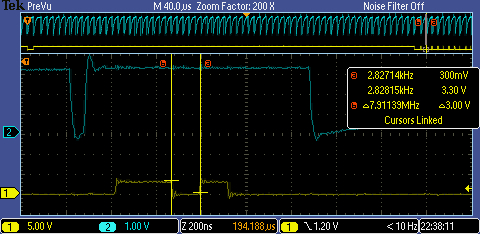
\includegraphics{TEK00001}
    \caption{A context switch}
    \label{fig:context-switch}
  \end{figure}
  \begin{figure}
    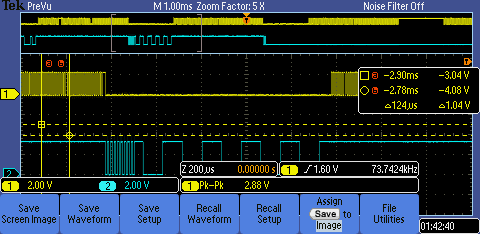
\includegraphics{TEK00000}
    \caption{Retrieving data from the UART FIFO. The blue line
      represents the UART consumer thread consuming UART data from the
      FIFO, the yellow line represents all other threads. You can
      clearly see the UART consumer thread retrieving data in the FIFO
      in quick succession, and then waiting for real-time data to
      arrive}
    \label{fig:uart-consumer}
  \end{figure}

\item Measurement of the Thread-Switch Time:

  The thread-switch takes less than 7$\mu$s to complete.
\item Reference \cref{fig:context-switch,fig:uart-consumer}.
\item This is what the circular linked list looks like before, after,
  and during a thread switch. The TCB pointed to by
  \verb|os_running_threads| circulates through the TCB data
  structures, as shown in \verb|$12| by the \verb|next| TCB variable.

\begin{verbatim}
  (gdb) p *os_running_threads
$9 = {
  sp = 0x200008a0 <OS_PROGRAM_STACKS+732>,
  next = 0x2000058c <OS_THREADS+56>,
  prev = 0x200005a8 <OS_THREADS+84>,
  id = 1,
  entry_point = 0x6e1 <uart_consumer>,
  status = THREAD_RUNNING,
  sleep_timer = 0
}
(gdb) p *os_running_threads->next
$10 = {
  sp = 0x20000a30 <OS_PROGRAM_STACKS+1132>,
  next = 0x200005a8 <OS_THREADS+84>,
  prev = 0x20000570 <OS_THREADS+28>,
  id = 2,
  entry_point = 0x651 <Thread2>,
  status = THREAD_RUNNING,
  sleep_timer = 0
}
(gdb) p *os_running_threads->next->next
$11 = {
  sp = 0x20000bc0 <OS_PROGRAM_STACKS+1532>,
  next = 0x20000570 <OS_THREADS+28>,
  prev = 0x2000058c <OS_THREADS+56>,
  id = 3,
  entry_point = 0x619 <Thread1>,
  status = THREAD_RUNNING,
  sleep_timer = 0
}
(gdb) p *os_running_threads->next->next->next
$12 = {
  sp = 0x200008a0 <OS_PROGRAM_STACKS+732>,
  next = 0x2000058c <OS_THREADS+56>,
  prev = 0x200005a8 <OS_THREADS+84>,
  id = 1,
  entry_point = 0x6e1 <uart_consumer>,
  status = THREAD_RUNNING,
  sleep_timer = 0
}
(gdb)
\end{verbatim}

\item  Reference \cref{tab:fifo-perf}.
  \begin{table}[h]
    \centering
    \begin{tabular}[H]{c|c|c|c|c}
           & 32 & 64 & 128 & 256 \\ \hline
      500  & 8  & 4  & 2   & 0   \\ \hline
      1000 & 6  & 3  & 0   & 0   \\ \hline
    \end{tabular}
    \caption{Context Switch Frequency (Hz) vs. UART Buffer FIFO Overwrites}
    \label{tab:fifo-perf}
  \end{table}
\item Reference \cref{tab:debugging-instruments-perf}.
  \begin{table}[h]
    \centering
    \begin{tabular}[H]{c|c}
      With Debugging Instruments & 1224 \\ \hline
      Without Debugging Instruments & 12300 \\
    \end{tabular}
    \caption{Context Switch Frequency (Hz) vs. UART Buffer FIFO Overwrites}
    \label{tab:debugging-instruments-perf}
  \end{table}
  The value of \verb|PIDWork| without debugging instruments is
    12300, the value with debugging instruments is 1224.
\end{enumerate}

\section{Analysis and Discussion}
\begin{enumerate}[1)]
\item Why did the time jitter in the lab manual's solution jump from 4
  to 6 μs when interpreter I/O occurrs? \\
  When I/O interrupt occurs, the uart handler interrupts normal
  program execution. This delays the completion time of the program's
  work, quantified as jitter.
\item Justify why Task 3 has no time jitter on its ADC sampling. \\
  Task 3 has no jitter because a hardware interrupt invokes the task.
\item There are four (or more) interrupts in this system DAS, ADC,
  Select, and SysTick (thread switch). Justify your choice of hardware
  priorities in the NVIC? \\
  All of the tasks besides \verb|PendSV_Handler| are the same
  priority. This is because the queueing of interrupts was not
  detrimental to our program execution during
  testing. \verb|PendSV_Handler| is the lowest interrupt priority so
  that it will only execute a context switch after all queued
  interrupts have completed.
\item Explain what happens if your stack size is too small. How could
  you detect stack overflow? How could you prevent stack overflow from
  crashing the OS? \\
  The effects of having too small a stack size are dependent on
  multiple factors. The most important dependent factor of your system
  is the location of your stack relative to other memory
  regions. Since the stack grows down on the Cortex M4, the only
  region in danger during a stack overflow is the region directly
  below the stack. If you have arranged your system like this !!TODO
  unsafe\_stack.jpg!! you can expect your data to be overwritten with
  stack contents. If instead you arrange your stack like this !!ToDO
  safe\_stack.jpg!! pointing your loaded stack at a somewhat safer
  region of memory such as memory-mapped I/O, you will only lose the
  ability to read back what you pushed that was beyond the
  capacity of the stack. \\
  In both cases, program behavior will deviate from the intended
  course sooner or later. The results could be inaccurate data or a
  full system crash. \\
  Prevention of stack overflow comes from confidence due to testing
  before you need your stack to not overflow. You can determine the
  maximum possible size of your stack through desk checking or static
  analysis. Trial-and-error runs whereby you place a 'magic cookie' at
  the end of your stack + 1 and examine the cookie at the end of
  program execution. If the cookie's data has been overwritten, you
  are using more stack space than you thought. Increase the size of
  your stack and try again until your magic cookie remains. This is
  not as thorough as static analysis, which calculates all possibly
  execution paths of your program, unless the cookie analysis occurs
  after the most rigorous testing your program will ever endure.
\item Both Consumer and Display have an \verb|OS_Kill()| at the end. Do these
  \verb|OS_Kill|s always execute, sometime execute, or never execute?
  Explain. \\
  I have no idea what you're referencing or what you're talking
  about. Please refer to a specific procedure within the
  document. Neither the Consumer nor the Display threads you mentioned
  contain \verb|OS_Kill()|. I cannot answer this question otherwise. Please
  be more clear in the future!
\item The interaction between the producer and consumer is
  deterministic. What does deterministic mean? Assume for this
  question that the \verb|OS_Fifo| loses data when it has 5 elements, but
  loses no data when it has 6 elements. What does this tell you about
  the timing of the consumer plus display? \\
  Deterministic means ``causally determined and not subject to random
  chance.'' The timing protocol between the lcd and the M4 will always
  occur at a set tempo. As a result the time it takes to transfer $n$
  chars to the lcd is \emph{deterministic}. If the Fifo is losing data
  with less than 6 elements, we can infer the exchange between the
  consumer and its display takes at least as long as it takes for 6
  chars to enter the Fifo.
\item Without going back and actually measuring it, do you think the
  Consumer ever waits when it calls \verb|OS_MailBox_Send|? \\
  No, the Consumer takes enough time during its communication with the
  lcd that the Producer will populate the Fifo before the Consumer
  invokes \verb|OS_MailBox_Send|.
\end{enumerate}

\end{document}
